\documentclass{article}
\usepackage{graphicx} % Required for inserting images

\title{Sistemi Operativi 1}
\author{Riccardo Cara}


\begin{document}
\maketitle
\tableofcontents
\newpage

\section{Introduzione}

    Un \textit{sistema operativo} è un software che si occupa di gestire le risorse hardware e fornire software di base che cambiano in base allo scopo del dispositivo.
    il sistema operativo si occupa di:

    \begin{itemize}
        \item \textbf{gestire le risorse hardware} gestire le risose fisiche condivise per raggiungere equità e efficenza
        \item \textbf{virtualizzare delle risorse} per dare alle applicazioni l'illusione di avere risorse infinite, altrimenti.
        \item \textbf{interfacciare hardware e software} permette agli utenti di interagire con le risorse hardware senza controllarle direttamente.
    \end{itemize}
    %
    e viene diviso in due parti:

    \begin{itemize}
        \item \textbf{software di sistema}:
        tutti i software che non sono il kernel

        \item \textbf{kernel}:
        il nucleo dell'OS e si occupa di:
        
            \begin{itemize}
                \item \textbf{interfaccia hardware}
                interfacciare  i software con l'hardware

                \item \textbf{gestione della memoria}
                si occupa di distribuire la ram (Random Access Memory)
                
                \item \textbf{gestione dei processi}
                si occupa della gestione del tempo e quindi permette il multitasking
                
                \item \textbf{gestione dispositivi}
            \end{itemize}
            %
            un software effettua delle system calls ("syscall" per chi ha studiato assembly), il kernel traduce le chiamate in serie di comandi e le invia alla cpu.
        
        
    \end{itemize}

\section{Un sistema computerizzato}

    {\centering 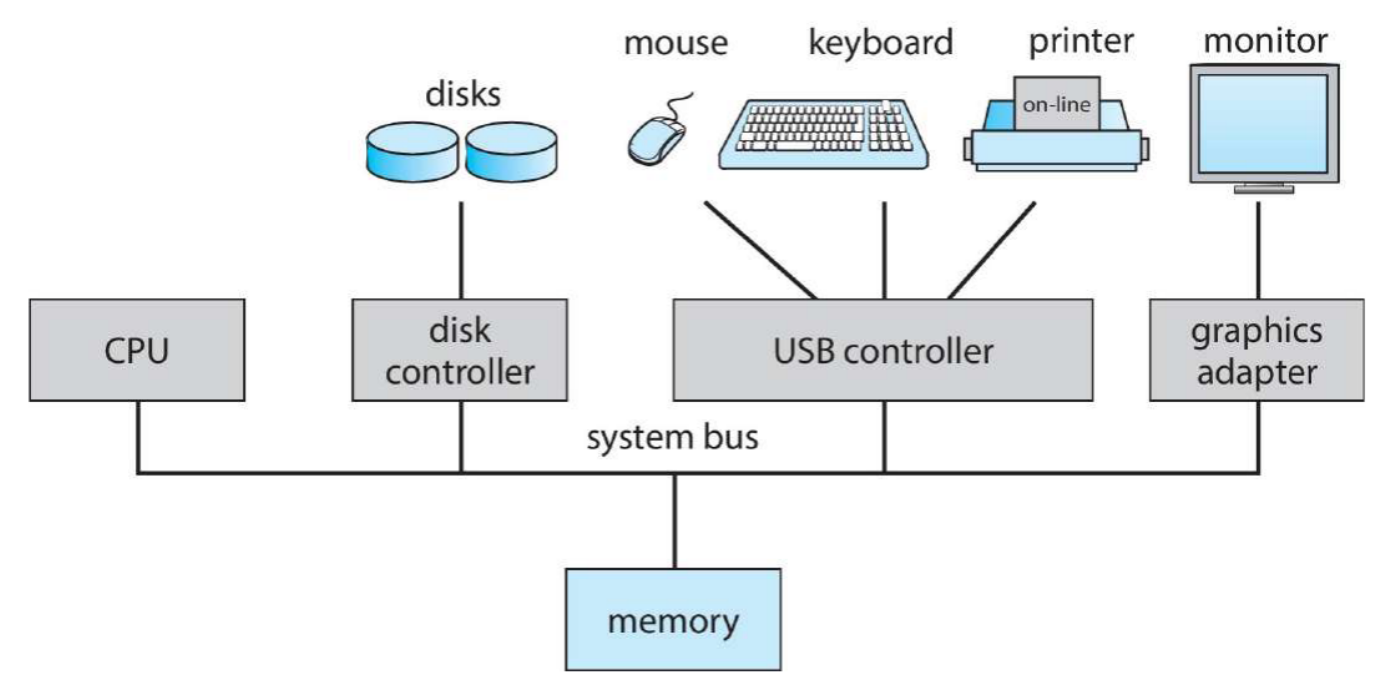
\includegraphics[width=0.8\textwidth]{immagini/immagine.png}}
    
    questo è lo schema di un computer, si può osservare che esso è composto da più componenti connessi tra loro tramite un bus di sistema che permette ai componenti del computer di comunicare tra loro. I componenti sono:

    \begin{itemize}

        \item \textit{CPU}
         la parte che esegue le computazioni

        \item\textit{memoria principale}
        immagazzina dati e istruzioni usati dalla CPU, è condivisa tra CPU e dispositivi I/O

        \item\textit{dispositivi I/O}
        sono le periferiche, ovvero i dispositivi che permettono al computer di comunicare (monitor, stampante, mouse, tastiera,...)

    \end{itemize}

    
    \subsection{Architettura di un computer}
    L'architettura di un computer è concettualmente identica tra Personal Computers, servers, smartphones ecc... basato sul concetto di programma memorizzato, ovvero un computer che immagazzina i dati e le istruzioni dei programmi sullo stesso spazio di memoria, prima di questa architettura, le istruzioni dei programmi e i dati erano salvati su spazi di memoria distinti, basti pensare a quando per cambiare programma si doveva cambiare scheda fisica. (non ne sono sicuro, forse era in un film, comunque il concetto è quello :D ).


    {\centering 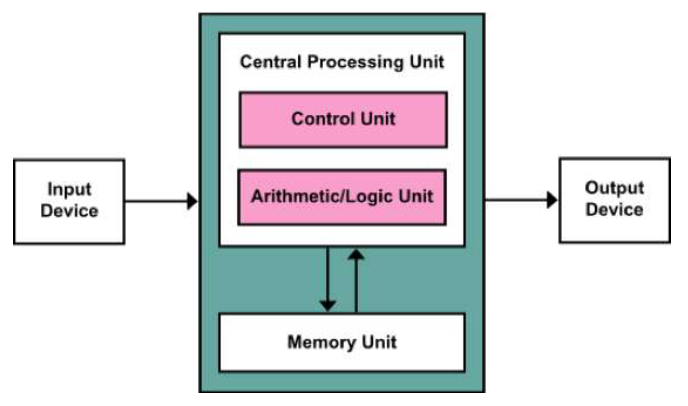
\includegraphics[width=0.8\textwidth]{immagini/architettura von neuman.png}}

    In questo tipo di architettura, la CPU esegue le operazioni in maniera sequenziale usando registri interni mentre la memoria contiene le istruzioni e i dati.
    \paragraph{CPU} esegue tre passi in maniera ciclica:
    \begin{enumerate}
        \item \textbf{Fetch}: raccoglie l'istruzione dal Program Counter (un registro di memoria speciale della cpu)
        \item \textbf{Decode}: interpreta l'istruzione fetchata
        \item \textbf{Execute}: esegue l'istruzione fetchata
    \end{enumerate}
    la CPU può essere a processore singolo o a processori multipli, la differenza più grande è che la cpu a processori multipli incrementa il throughput, ovvero, nello stesso periodo di tempo, la cpu a processori multipli da in output una mole di dati maggiore rispetto al processore singolo in questo corso ci concentreremo sui systemi a processore singolo. La CPU possiede delle istruzioni, l'insieme di istruzioni viene definito dal linguaggio macchina. Le istruzioni in linguaggio macchina sono composte da un operatore (op code), zero o più operandi rappresentanti registri di memoria o indirizzi di memoria.

    \paragraph{Memoria}
    in un Sistema computerizzato ci sono molte memorie, registri di memoria, cache, RAM, spazi di archiviazione(HDD, SSD) ecc... queste memorie hanno un sistema gerarchico a livello di costi, capacità di memoria e a livello di tempo impiegato per accedervi:
    {\centering 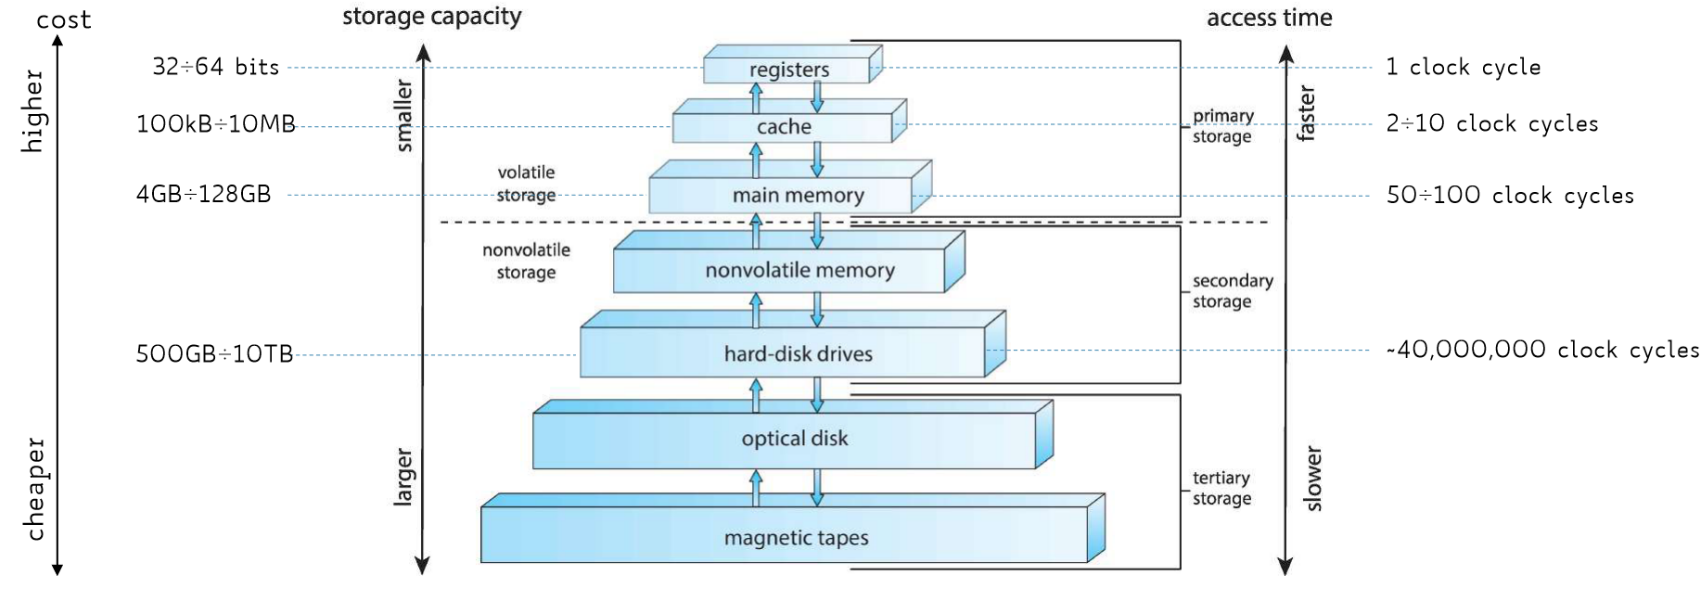
\includegraphics[width=0.8\textwidth]{immagini/gerarchia memorie.png}}
    le memorie sono divise in due sottogruppi:
    \begin{enumerate}
        \item \textbf{registri e cache}: sono gestiti dall'architettura
        \item \textbf{memoria principale, memoria non volatile, spazi di archiviazione}: sono gestiti dal sistema operativo
    \end{enumerate}
    \subsection{Bus di sistema}
    i bus di sistema sono 3:
    \begin{itemize}
        \item \textbf{Data Bus}: porta l'informazione
        \item \textbf{Address Bus}: determina dove l'informazione va inviata
        \item \textbf{Control Bus}: determina quale operazione viene effettuata
    \end{itemize}
    Se il control bus è condiviso tra memoria e dispositivi di I/O di cui si parlerà nella prossima sezione, si utilizzerà una linea speciale chiamata"\textbf{M/\#io}" ed indica se la CPU vuole comunicare con la memoria o con un dispositivo I/O.
    \subsection{dispositivi I/O}
    i dispositivi input output, sono divisi in 2 parti, il dispositivo in se e il device controller, ovvero un chip che permette di controllare una famiglia di device controller:
    \begin{itemize}
        \item SATA controller: controlla i dischi SATA
        \item IDE controller: controlla i dischi IDE
        \item usb controller: controlla i dispositivi USB
        \item PCI bus controller: controlla i dispositivi connessi al bus PCI
        \item ...
    \end{itemize}
    il sistema computerizzato, comunica con gli elementi I/O tramite dei software chiamati driver: SATA driver, IDE driver, USB driver, PCI bus driver ecc... I dispositivi I/O hanno dei registri dedicati con cui comunicare con il sistema computerizzato.
    \begin{itemize}
        \item registri di stato: registro in cui viene salvato lo stato del dispositivo(attende l'input, occupato, errore, transazione completata, idle, ecc...)
        \item registri di controllo/configurazione: usato dalla CPU per configurare e controllare il dispositivo
        \item registri dei dati: usato per leggere o inviare dati dal/al dispositivo I/O
    \end{itemize}
    La CPU può comuicare con i dispositivi I/O in due modi:
    \begin{itemize}
        \item Port-mapped I/O si riferisce ai registri dei controller tarmite spazio di indirizzi I/O separato.
        \begin{itemize}
            \item il registro di ogni device controller è mappato ad una porta (indirizzo) specifica durante il boot
            \item necessita di istruzioni della CPU speciali (IN per leggere dal dispositivo I/O, OUT per scriverci)
            \item non necessita di interpellare M/\#IO per le istruzioni IN, OUT poichè sono solo per i dispositivi I/O e non confondibili con altre istruzioni per la memoria.
        \end{itemize}
        
        \item memory mapped I/O i registri dei controller vengono mappati sugli stessi indirizzi usati per i registri di memoria.
        \begin{itemize}
            \item non necessita di istruzioni speciali
            \item le porte dei dispositivi I/O sono viste come normali indirizzi di memoria mappati nella RAM
            \item per accedere ai registri dei dispositivi I/O vengono usate istruzioni simili a MOV
            \item M/\#IO indica sempre che gli indirizzi richiesti dalla CPU appartengono alla memoria 
        \end{itemize}
    \end{itemize}

\end{document}
